\documentclass[a4paper]{article} % template
\usepackage{fullpage}
\usepackage[utf8]{inputenc}
\usepackage{booktabs}
\usepackage{graphicx} % include pictures and tables
\usepackage{bigstrut} % for tables
\usepackage{float} % to force tables here
\usepackage{verbatim} % to comment
\usepackage{parskip} % to have no indentation in paras
\usepackage{amsmath} % for math
\usepackage{appendix} % to put appendix
\usepackage{multirow} % to put merge and centered rows
\usepackage{rotating}
\usepackage[hidelinks]{hyperref} %to make clickable links
\hypersetup{
  colorlinks=true}
\usepackage{rotfloat} % to put the sideways image here
\usepackage[export]{adjustbox} % to put a frame
\usepackage{setspace}


\begin{document}

\begin{titlepage}

\centering
\vspace{5cm}

\includegraphics[width=0.5\textwidth]{tuelogo}\\
{\scshape\Large School of Industrial Engineering \par}

\vspace{5cm}

	{\scshape\LARGE Report on the BPM Game\par}
	22/12/2017
	\vspace{1.5cm}
	\vfill
	{\huge\bfseries Group 30\par}
	\vspace{1.5cm}
	{\Large\itshape Bhoomica Nataraja	1282832\\
Hans Wammes	871125\\
Ilse Peeters	842836\\
Nitish Singh	1283901\\
     \par}
     \vfill
     
     
\end{titlepage}
\doublespacing
\tableofcontents
\singlespacing
\newpage
\section{Process Model}
% Table generated by Excel2LaTeX from sheet 'Sheet2'
\begin{table}[htbp]
  \centering
  
    \begin{tabular}{|c|c|c|}
    \hline
    \textbf{Role} & \textbf{Resources} & \textbf{Prioritized?} \bigstrut\\
    \hline
    \multirow{4}[8]{*}{risk management} & Frank & Yes \bigstrut\\
\cline{2-3}          & Minh  & Yes \bigstrut\\
\cline{2-3}          & Murray & No \bigstrut\\
\cline{2-3}          & Cecily & No \bigstrut\\
    \hline
    \multirow{2}[4]{*}{customer contact} & Ismael & Yes \bigstrut\\
\cline{2-3}          & Madeline & No \bigstrut\\
    \hline
    \multirow{2}[4]{*}{administration} & Rafael & Yes \bigstrut\\
\cline{2-3}          & Marisela & No \bigstrut\\
    \hline
    \multirow{2}[4]{*}{senior risk management} & Cecily & Yes \bigstrut\\
\cline{2-3}          & Murray & No \bigstrut\\
    \hline
    \multirow{3}[6]{*}{finance} & Murray & Yes \bigstrut\\
\cline{2-3}          & Cecily & No \bigstrut\\
\cline{2-3}          & Minh  & No \bigstrut\\
    \hline
    \end{tabular}%
  \label{tab:resource_allocation}%
  \caption{Resource Allocation}
\end{table}%

The Process model is as shown in Figure \ref{BPMNmodel}.
\begin{sidewaysfigure}[H]
\begin{center}
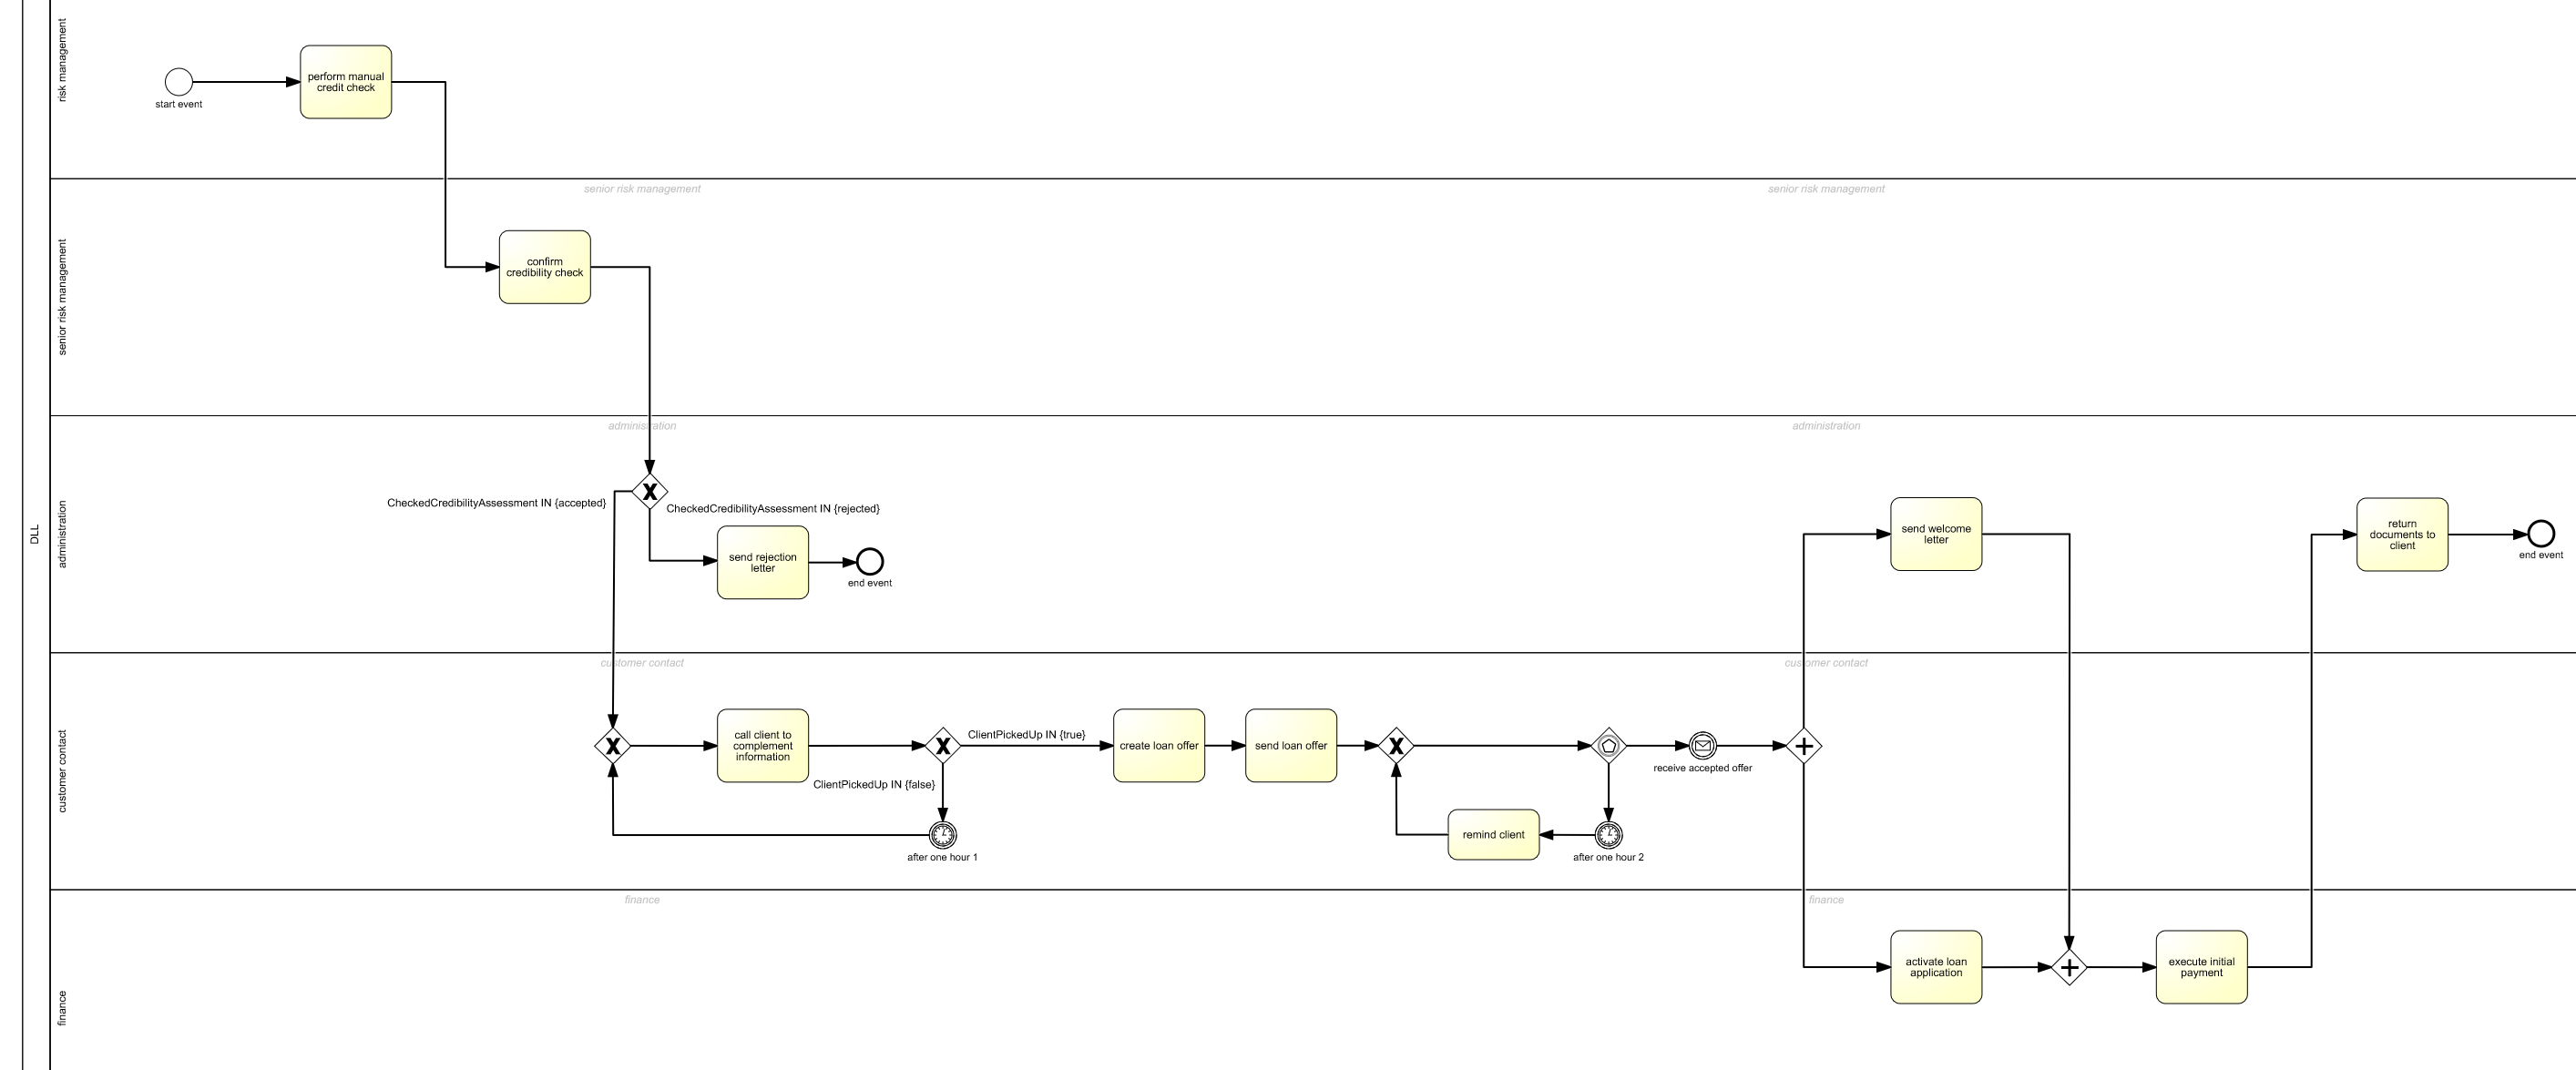
\includegraphics[scale=0.3,frame]{modelx.png}
%[width=1.1\textwidth]
\caption{BPMN Process Model}

\end{center}
\label{BPMNmodel}
\end{sidewaysfigure}


\section{Product-Based Redesign}
The aim of this \textit{Product-based redesign} is to radically rethink how the process of executing a loan application can be created. This method has been developed to “design processes that produce informational products” \cite{dumas2013}. Therefore, the product-based redesign can be used for the process to decide whether a client should be given a loan or not. Although, how the process goes on after the decision has been made whether a client will receive a loan, is not taken into account by the product-based redesign. As presented by Dumas et al. (2013) \cite{dumas2013}, the four stages for the redesign are: (1) scoping; (2) analysis; (3) design; (4) evaluation. 

In the scoping phase, the decision is made to focus on the business process of selling a loan. The performance targets are service time, waiting time, costs and customer satisfaction. 

Within the second phase, the analysis, a product data model is designed to represent the elements of the process, their dependencies and their processing logic. The product data model is presented in figure \ref{PDM1}. The information elements are chosen with the criteria of Dumas et al. (2013)\cite{dumas2013}. The list of activities is as follows:\\\\

\begin{figure}[H]
\centering
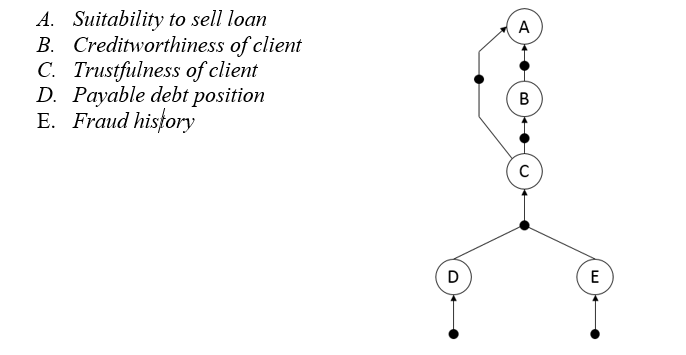
\includegraphics[scale=0.8, frame]{PDM1}
\caption{The sell loan product data model}
\label{PDM1}
\end{figure}
When \textit{Payable debt position} or \textit{Fraud history} is negative, the client can be trusted to sell a loan to. When the trustfulness of a client is low, the client will not be suitable to sell a loan to. When the trustfulness of the client is high, the creditworthiness of the client is determined, after which the suitability for the selling of a loan will be decided.

The three steps we analyzed to identify all the relevant characteristics are the source analysis, the production analysis and the fraction analysis. The source analysis presents that the most reliable and fast way to receive information about the \textit{payable debt position} is the BKR \cite{ABN} (in comparison with directly requesting information from the client or other companies). To receive information about the \textit{fraud history} of a potential client, the EVA would be most reliable and fast as well.

Both \textit{Fraud history} and \textit{Payable debt position} need the same time and costs, automatically and manually. This means that it does not matter which task to do first. Since both the tasks do not need further information, they can be performed in parallel.

The third step is the design phase. This resulted in the process model of figure \ref{BPM1}. As argued before, within the product-based redesign we just restructured the first part of the process. With the results of the redesign, we decided to check for \textit{payable debt position} and \textit{fraud history}  in  parallel. When we applied this to our BPMN model – as automated tasks - both the processing time and customer satisfaction decreased. Also, when we performed the automated BKR and EVA, a considerable number of cases still performed the manual check. This, together with the higher customer satisfaction of the manually performed BKR and EVA, led to our decision of still performing the \textit{manual credit check} at the beginning.

Also, it is presented in the product based redesign the possibility to go from \textit{trustfulness of client} directly towards \textit{suitability to sell loan}, when a client is not trustworthy. This sequence was not implemented within the BPMN model, because the assignment stated that we should also double check the credibility. This decision is appropriate because it is important to be sure about whether someone is trustworthy or not. Therefore, it was decided to always confirm the credibility within our BPMN model.\\
\begin{figure}[H]
\centering
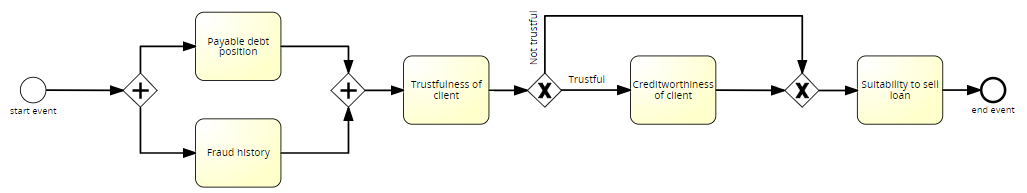
\includegraphics[scale=0.65]{BPM1}
\caption{The sell loan process model}
\label{BPM1}
\end{figure}

Once the design of the \textit{suitability to sell loan} was done, further procedures were designed in a similar approach. The BPMN model derived from the product based design has almost all the processes in a sequence.\\

\begin{figure}[H]
\centering
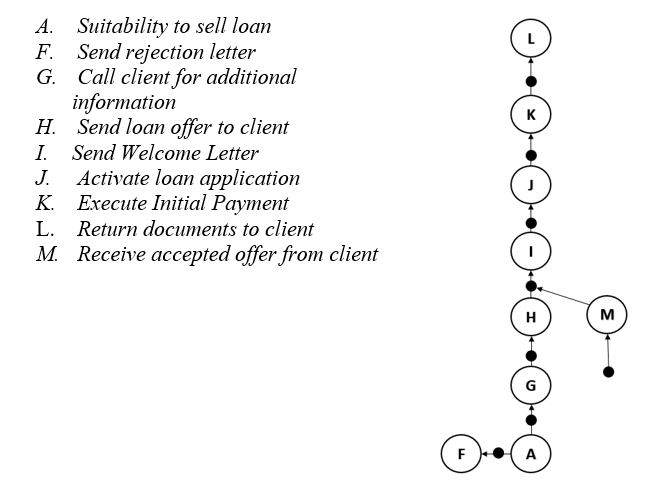
\includegraphics[scale=0.8, frame]{PDM2}
\caption{Product Data Model after determining suitability}
\label{PDM2}
\end{figure}
The features of the credibility assessment lead us to implement a model with the right tasks although the product based design was not implemented. Some of the aspects related to the administration procedure after checking suitability to sell loan were almost sequential (figure \ref{BPM2}), while most of the tasks implemented in the final BPMN model employs parallelism. In conclusion, the product-based redesign showed us some possible changes, however, we did not implement those changes since we value customer satisfaction and the fairness of our decision. \\

\begin{figure}[H]
\centering
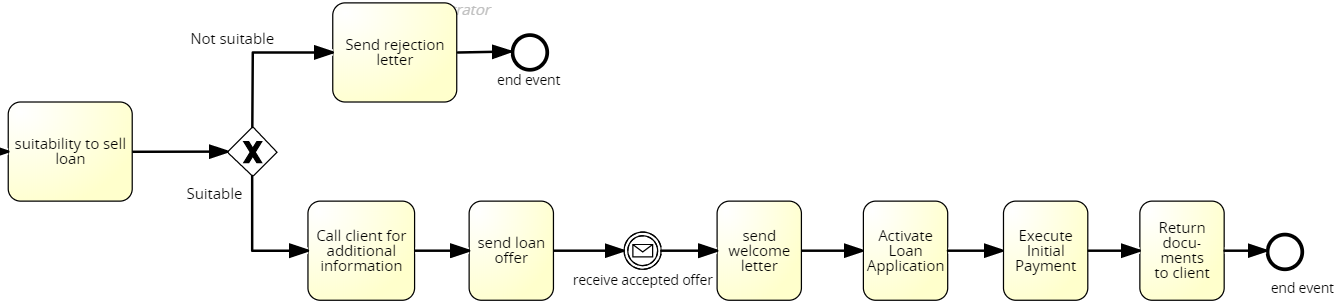
\includegraphics[scale=0.5]{BPM2}
\caption{BPMN model derived from product based design}
\label{BPM2}
\end{figure}

\section{Redesign Heuristics}
The following sections explain the heuristics employed in our BPMN model and the following table summarizes the effect of the heuristics on the performance dimensions of the Devil’s Quadrangle.

% Table generated by Excel2LaTeX from sheet 'Group'
\begin{table}[H]
  \centering
  
    \begin{tabular}{|p{8.715em}|c|c|c|c|c|}
    \hline
    \textbf{Category} & \textbf{Heuristics} & \textbf{Time} & \textbf{Cost} & \textbf{Quality} & \textbf{Flexibility} \bigstrut\\
    \hline
    Business Process Behavior & Parallelism & +     & -     & .     & - \bigstrut\\
    \hline
    Technology & Activity automation & +     & -     & +     & - \bigstrut\\
    \hline
    Organization Structure & Flexible assignment & +     & -     & .     & + \bigstrut\\
    \hline
    Organization Population & Extra resources & +     & -     & .     & + \bigstrut\\
    \hline
    \end{tabular}%
  \label{tab:devils_qudrangle}%
  \caption{Devil's Quadrangle}
\end{table}%

\subsection{Heuristic 1: Parallelism – “Consider whether activities may be executed in parallel”}
At first, the ‘call client to complement information’ and ‘create loan offer’ activity had been modelled in parallel to improve the throughput time. This was assumed to be feasible as the input for ‘create loan offer’ is not generated by the ‘call client to complement information’ activity. In the end, however, these activities were placed subsequently since both activities are performed by the same role, reducing the possible improvements due to resource limitations. If the resources are scarce, placing the activities in parallel increased the waiting time for other cases since multiple employees with the same skills were working on only one case instead of working on multiple cases.

Parallelism is used in the placement of the activities ‘send welcome letter’ and ‘activate loan application’ (shown in figure \ref{H2}) as the input of either activity is not generated by the other. Additionally, both activities are executed by different roles, which improved the processing time with the application of this heuristic. If these activities are not placed in parallel, one employee might be idle waiting for the other to complete the first task if there are no other cases which needs his attention. Moreover, both the activities have equal service times (10 minutes) and ideally finish at the same time if the respective resources are available. Further analysis of the time taken was measured through Disco by dividing the total time taken for the activity by its case frequency.\\

% Table generated by Excel2LaTeX from sheet 'Sheet3'
\begin{table}[htbp]
  \centering
  
    \begin{tabular}{|r|r|r|}
    \hline
          & \multicolumn{2}{p{20.715em}|}{Time taken in minutes obtained from Disco} \bigstrut\\
    \hline
    Activity & Before parallelism & After parallelism \bigstrut\\
    \hline
    Send Welcome letter + Activate loan application & 10.73 + 7.2 = 17.93 & Max (8.29 , 9.09) = 9.09 \bigstrut\\
    \hline
    \end{tabular}%
    \caption{Time consumed before and after the application of Parallelism heuristic}
  \label{tab:parallelism_heuristic}%
\end{table}%

\begin{figure}
\centering
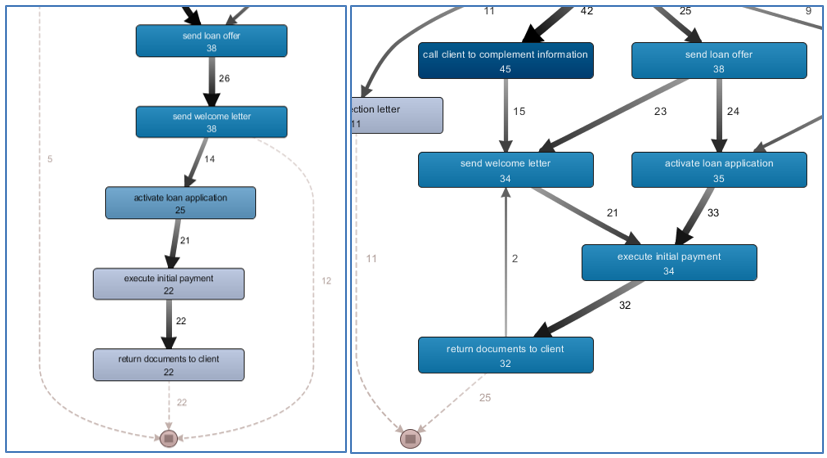
\includegraphics[scale=1]{h1}
\caption{Comparison between before and after application of Parallelism}
\label{H1}
\end{figure}

\begin{figure}
\centering
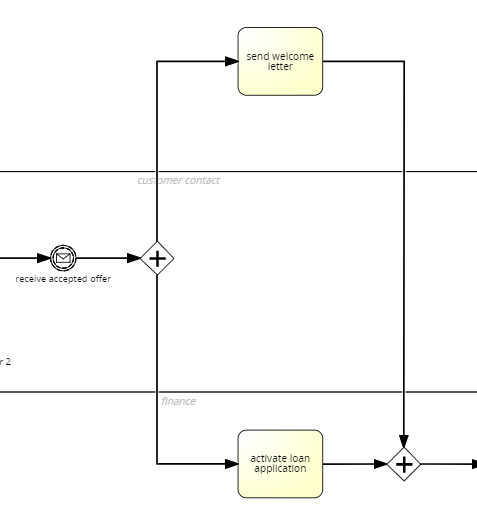
\includegraphics[scale=0.4]{h2}
\caption{Fragment of the process model with Parallelism}
\label{H2}
\end{figure}

\subsection{Heuristic 2: Activity Automation – “Consider automating activities”}
The technology heuristic “activity automation” does not take place within our model. While we considered to perform the BKR check; EVA check and credibility check automated in different manners, we decided not to change the manual credit check into an automated one. An example of a fragment of the model we applied is presented in figure \ref{H3}.

\begin{figure}[H]
\centering
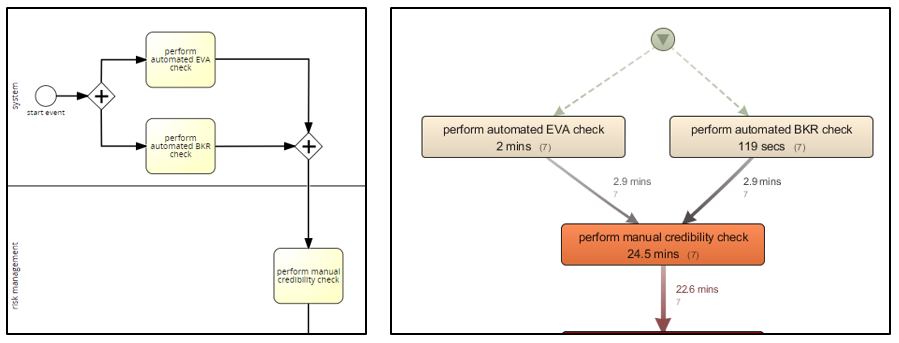
\includegraphics[scale=0.7]{h3}
\caption{Fragment process model automation}
\label{H3}
\end{figure}

In line with Dumas et al. (2013)\cite{dumas2013}, we found a decrease in quality for this model. With this model, a gradual decrease in the customer satisfaction and increase in the waiting time were observed. This could be caused by the fact that the customer expects manual evaluation of his credibility. This was visible at the execution log and on the simulation graphs. Additionally, after the automated EVA and BKR checks a considerable number of times a manual check followed and these two tasks consumed 2 minutes and 119 seconds respectively for 7 cases. The system ideally should have taken 0 seconds to perform the automated tasks, therefore, we decided not to perform the EVA and BKR check automated, but manually.

\subsection{Heuristic 3: Flexible assignment – “Assign resources in such a way that maximal flexibility is preserved for the near future” }

The model consists of many resources and hence it was found necessary to employ some of the organizational heuristics to achieve better performance as well as balance the total costs of the organization. Flexibility assignment relates to the structure of the organization mostly the allocation of the resources in accordance with Dumas et al.(2013)\cite{dumas2013}.

Initially single resources were allocated to certain tasks to evaluate the performance measures such as the waiting time and sojourn times. Many resources were hired and fired throughout the process in order to finalize a set of resources that would be a part of the organization in the final model. System was involved in the initial models and was removed later as it contributed to decrease in customer satisfaction.\\

\begin{figure}[H]
\centering
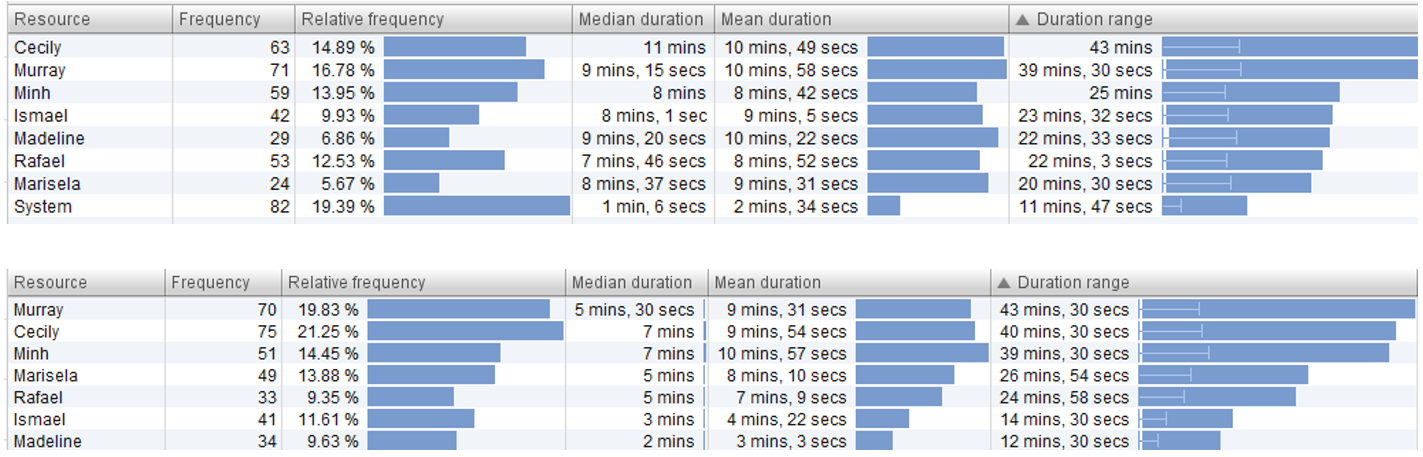
\includegraphics[scale=0.6]{h4}
\caption{Removal of automated tasks i.e., removal of system didn’t affect the performance of the resources at an intermediate modeling stage}
\label{H4}
\end{figure}

More than one resource of the same specialization are assigned to perform a task so that general resources can execute other tasks. In addition, the resources are prioritized so that every task has a dedicated resource. Assigning specialized resources could reduce the probability of bottlenecks due to the unavailability of the resources i.e., it is less probable that the execution of a job has to await the availability of a specific resource, thus reducing the overall queue time. Therefore, the cycle time of a business process should improve as the flexibility increases and the resources perform tasks (manual credit check) in parallel when more than one job are being processed at the same time.

It was observed that not prioritizing the resources caused two resources (Murray and Madeline) performing the same tasks of customer contact at the same time. After observing the performance of each worker and assigning the priority, the work quality improved in turn improving the customer satisfaction.\\

\subsection{Heuristic 4: Extra resources – “If capacity is not sufficient, consider increasing the number of resources”}
Another heuristic, extra resources, relating to the organizational population was employed. Here the cost was taken into consideration when administrative tasks came into picture. Resources from the administration department is required to perform 3 tasks in the whole process – 1 when the loan application is rejected and 2 when the application is accepted. Hence, it was decided to hire a contractor rather than employing a permanent resource for these intermittent tasks.

Employing additional resources also contributes to flexibility. A contractor has been hired for the administration tasks as the waiting times increased only for a few cases. After hiring the contractor, it was observed that the cycle time of the process gradually improved and the queue time decreased, since the probability that a case has to wait for a resource being available decreased. Also, this change did not result in any spike in the cost graph.

Another advantage of employing an extra resource is that resources can work on multiple cases at a time in contrast with the conventional method of having single resource who would be engaged in one case while the other cases would be waiting until that resource is available. So hiring extra resources would be an added value benefit not only in terms of the performance measures but also to implement parallelism heuristic.

\section{Quantitative Analysis}
\subsection{Waiting Times}
% Table generated by Excel2LaTeX from sheet 'Quant Analysis'
\begin{table}[H]
  \centering
  
    \begin{tabular}{|l|r|r|r|}
    \hline
    Activity & \multicolumn{1}{p{9.355em}|}{Waiting Time\newline{}(From Disco) (In Mins)} & \multicolumn{1}{l|}{No. of Cases} & \multicolumn{1}{l|}{Actual Waiting Time/Case} \bigstrut\\
    \hline
    perform manual credit check & 0     & 55    & 0 \bigstrut\\
    \hline
    confirm credibility check & 258   & 55    & 4.690909091 \bigstrut\\
    \hline
    send rejection letter & 2.5   & 16    & 0.15625 \bigstrut\\
    \hline
    call client to complement information & 14.1  & 39    & 0.361538462 \bigstrut\\
    \hline
    create loan offer & -     & -     & - \bigstrut\\
    \hline
    send loan offer & 21.6  & 30    & 0.72 \bigstrut\\
    \hline
    remind client & 6     & 12    & 0.5 \bigstrut\\
    \hline
    send welcome letter & 667   & 23    & 29 \bigstrut\\
    \hline
    activate loan application & 1608  & 49    & 32.81632653 \bigstrut\\
    \hline
    execute initial payment & 924   & 29    & 31.86206897 \bigstrut\\
    \hline
    return documents to client & 216   & 31    & 6.967741935 \bigstrut\\
    \hline
    \end{tabular}%
    \caption{Waiting Times from Disco}
  \label{tab:wait_time_from_disco}%
\end{table}%


\subsection{Activity Cycle Time and Processing Times}

% Table generated by Excel2LaTeX from sheet 'Sheet1'
\begin{table}[H]
  \centering
  %\caption{Add caption}
    \begin{tabular}{|l|r|r|}
    \hline
    Activity & \multicolumn{1}{l|}{Cycle Time} & \multicolumn{1}{l|}{Service Time/Processing Time} \bigstrut\\
    \hline
    perform manual credit check & 10.69090909 & 10.69090909 \bigstrut\\
    \hline
    confirm credibility check & 17.12727273 & 12.43636364 \bigstrut\\
    \hline
    send rejection letter & 6.711805556 & 6.555555556 \bigstrut\\
    \hline
    call client to complement information & 4.647252747 & 4.285714286 \bigstrut\\
    \hline
    create loan offer & \multicolumn{1}{l|}{-} & \multicolumn{1}{l|}{-} \bigstrut\\
    \hline
    send loan offer & 4.509473684 & 3.789473684 \bigstrut\\
    \hline
    remind client & 3.571428571 & 3.071428571 \bigstrut\\
    \hline
    send welcome letter & 37.29411765 & 8.294117647 \bigstrut\\
    \hline
    activate loan application & 41.90204082 & 9.085714286 \bigstrut\\
    \hline
    execute initial payment & 41.04956897 & 9.1875 \bigstrut\\
    \hline
    return documents to client & 14.46774194 & 7.5 \bigstrut\\
    \hline
    \end{tabular}%
    \caption{Activity cycle
times and processing times}
  \label{tab:addlabel}%
\end{table}%

\subsection{Sojourn Times}

%\begin{flushleft}
%\textbf{Sojourn Times for Variants 1, 2 and 3 from Execution %Logs}%
%\end{flushleft}
\subsubsection*{Sojourn Times for Variants 1, 2 and 3 from Execution Logs}
% Table generated by Excel2LaTeX from sheet 'Summary'
\begin{table}[H]
  \centering
  
    \begin{tabular}{|l|r|l|}
    \hline
    Variant & \multicolumn{1}{l|}{Number of Cases} & Sojourn Time(From Disco) \bigstrut\\
    \hline
    Variant 1 & 16    & 36 Minutes \bigstrut\\
    \hline
    Variant 2 & 7     & 96.5 Minutes \bigstrut\\
    \hline
    Variant 3 & 5     & 116.4 Minutes \bigstrut\\
    \hline
    \end{tabular}%
    \caption{Sojourn times from Disco}
  \label{tab:addlabel}%
\end{table}%




\begin{comment}

Cycle Time is calculated based on the visit frequencies to the activities in an XOR-split i.e.
\begin{center}
 \vspace{0.5cm}
 
 $ CT = \sum_{i=1}^{n} pi * Ti $ \\
\vspace{0.5cm}
 $p_{i}$ =Branching Probability\\
 $T_{i}$ = Cycle Time of nested fragments
 
 \end{center} 

In an AND-Gate the combined cycle time is determined by the slowest activity within the And join, i.e.,

\begin{center}
CT = Max($T_{1},T_{2},.....,T_{n}$)
\end{center}

Another recurrent case worth considering is the case where a fragment of a process
may be repeated multiple times. This situation is called rework.

\end{comment}
\begin{flushleft}
\textbf{Flow Analysis of Sojourn Times for Variants 1, 2 and 3}
\end{flushleft}
Sojourn Time or Cycle Time of a process is the average time it takes between the moment the process starts and the moment it completes.Cycle Time is calculated based on the visit frequencies to the activities in an XOR-split i.e.

\begin{equation}
\label{CTX}
CT = \sum_{i=1}^{n} pi*Ti
\end{equation}
\begin{itemize}
\item$p_{i}$ =Branching Probability
\item$T_{i}$ = Cycle Time of nested fragments
 \end{itemize}
 
In an AND-Gate the combined cycle time is determined by the slowest activity within the And join, i.e.,

\begin{equation}
\label{CTP}
CT = Max(T_{1},T_{2},.....,T_{n})
\end{equation}

Using flow analysis formulas mentioned above, sojourn time can be calculated for the 3 variants.

% Table generated by Excel2LaTeX from sheet 'Summary'
\begin{table}[H]
  \centering
  
    \begin{tabular}{|c|c|r|}
    \hline
    \multicolumn{1}{|l|}{Variant 1} & \multicolumn{1}{l|}{Type} & \multicolumn{1}{l|}{Activity Cycle Time(In Minutes)} \bigstrut\\
    \hline
    \multicolumn{1}{|l|}{perform manual credit check} & \multicolumn{1}{l|}{Sequential} & 10.69090909 \bigstrut\\
    \hline
    \multicolumn{1}{|l|}{confirm credibility check} & \multicolumn{1}{l|}{Sequential} & 17.12727273 \bigstrut\\
    \hline
    \multicolumn{1}{|l|}{send rejection letter} & \multicolumn{1}{l|}{Sequential} & 6.711805556 \bigstrut\\
    \hline
    \multicolumn{2}{|c|}{\textbf{Total Cycle Time}} & \textbf{34.52998737} \bigstrut\\
    \hline
    \end{tabular}%
    \caption{Flow Analysis for Variant 1}
  \label{tab:sojtime}%
\end{table}%

% Table generated by Excel2LaTeX from sheet 'Summary'
\begin{table}[H]
  \centering
  
    \begin{tabular}{|c|c|r|}
    \hline
    \multicolumn{1}{|l|}{Variant 2 \& 3} & \multicolumn{1}{l|}{Type} & \multicolumn{1}{l|}{Activity Cycle Time(In Minutes)} \bigstrut\\
    \hline
    \multicolumn{1}{|l|}{perform manual credit check} & \multicolumn{1}{l|}{Sequential} & 10.69090909 \bigstrut\\
    \hline
    \multicolumn{1}{|l|}{confirm credibility check} & \multicolumn{1}{l|}{Sequential} & 17.12727273 \bigstrut\\
    \hline
    \multicolumn{1}{|l|}{call client to complement information} & \multicolumn{1}{l|}{Sequential} & 4.647252747 \bigstrut\\
    \hline
    \multicolumn{1}{|l|}{send loan offer} & \multicolumn{1}{l|}{Sequential} & 4.509473684 \bigstrut\\
    \hline
    \multicolumn{1}{|l|}{send welcome letter} & \multicolumn{1}{l|}{Parallel(AND)} & 37.29411765 \bigstrut\\
    \hline
    \multicolumn{1}{|l|}{activate loan application} & \multicolumn{1}{l|}{Parallel(AND)} & \textbf{41.90204082} \bigstrut\\
    \hline
    \multicolumn{1}{|l|}{execute initial payment} & \multicolumn{1}{l|}{Sequential} & 41.04956897 \bigstrut\\
    \hline
    \multicolumn{1}{|l|}{return documents to client} & \multicolumn{1}{l|}{Sequential} & 14.46774194 \bigstrut\\
    \hline
    \multicolumn{2}{|c|}{\textbf{Total Cycle Time}} & \textbf{134.39426} \bigstrut\\
    \hline
    \end{tabular}%
    \caption{Flow Analysis for Variants 2 and 3}
  \label{tab:addlabel}%
\end{table}%

\subsection{Summary of Quantitative Analysis}
Flow analysis for our process model highlights certain similarities and certain differences in observed and intended behaviour of the model. The inter-arrival rates were drilled further to understand the different types of 'cases' or customers that arrive in the model. The 3 most frequent case types had a collective inter-arrival rate of about 2.5 cases / hr. After calculating service times via event logs on disco, a strong conformance was found between actual service times and service times described in the assignment, of course, there is a slight variation in observed values due to exponential distribution of the same. Furthermore, after observing the waiting times and consequently plotting activity cycle times, it can be seen that assigned resources work well in terms of processing times and wait times thus reducing the activity cycle times at different stages of the process model. There are however a few exceptions such as 'send welcome letter', 'activate loan application' and 'execute initial payment' which  have on an average a wait time of about 40 minutes, which is a potential area of improvement in the model. 

Sojourn times are calculated from execution logs for the 3 most frequent variants of our execution logs (Check appendix for a detailed description of the variants) and we compare it with the complete cycle time calculations using flow analysis rules and the values that we obtain as a result are fairly consistent. While, flow analysis provides a good idea on the processing times and waiting times in the model, it does not consider load-dependant tasks and may overlook the effect of an increase in resource contention, i.e. when the load goes up and resources remain constant, the waiting times increase. Furthermore, flow analysis tends to consider 'average' effects of the cases, i.e., effect on waiting times when customers arrive together or in groups is overlooked in flow analysis, however, in reality, it may have a compounded effect on the actual waiting time for a customer.

\section{Process Mining}
In order to improve the model, process mining  tool has been used throughout the project to analyze the performance of the model. By loading the simulation log of the latest model into ‘Disco’, a visual overview of the simulation log can be seen as shown in figure \ref{conformance}.

\begin{figure}
\centering
\includegraphics[scale=0.5,frame]{conformance}
\caption{Visual overview of simulation log}
\label{conformance}
\end{figure}

There are some noteworthy differences between the model generated from the simulation log and the implemented model. Going through the model, the first difference occurs after the activity ‘confirm credibility check’ is performed. According to the implemented model only the activities ‘send rejection letter’ and ‘call client to complement information’ are to be performed after the ‘confirm credibility check’ activity. Another significant difference is the absence of the activity ‘create loan offer’ in the simulated model. There are some cases in which the ‘execute initial payment’ activity started after the ‘activate loan application’ while the ‘send welcome letter’ activity was not finished yet. The aforementioned differences are discussed in the following sections.

\subsection{Difference 1: activity ‘send loan offer’ after ‘confirm credibility check’}
The logs from the simulation when filtered solely on cases in which the ‘send loan offer’ activity is performed straight after the ‘confirm credibility check’ activity, we noticed for almost every case that the ‘send loan offer’ and the ‘call client to complement information’ activities were performed in parallel. Since numerous similar cases occurred, these errors might be considered employee errors, implying the possibility of performing these activities in parallel. When further improving the model, this change should be taken into consideration.

\subsection{Difference 2: activity ‘remind client’ after ‘confirm credibility check’}
When checking the logs from the simulation, filtered on cases in which the ‘remind client’ activity is performed straight after the ‘confirm credibility check’ activity, it was noticed that for every case the ‘remind client’ activity is performed in parallel to the ‘call client to complement information’ and ‘send loan offer’ activities (as explained in Difference 1). However, we believe that the ‘remind client’ activity does not belong there at all. There is no reason to remind the client yet since no loan offer has been sent yet. In addition to this, one must wait one hour for an accepted offer before reminding the client. Given the frequency of the occurrence of these errors, it cannot be considered as a random error. Given the lack of logical reasons for this error to occur, we believe this might be an error caused by the BPM Game not being perfect yet.

\subsection{Difference 3: the absence of the ‘create loan offer’ activity}
In order to send the loan offer, a loan offer has to be created first. Since the required data for the ‘send loan offer’ activity is LoanOffer, which is produced by the ‘create loan offer’ activity, it cannot be that the ‘create loan offer’ activity is really skipped. Again, we believe this to be an error caused by the BPM Game not being perfect yet. When further improving this model, we would not take any action regarding this difference.

\subsection{Difference 4: the ‘execute initial payment’ activity started before the ‘send welcome letter’ activity has been performed}
Another observation made was that the finance team executed initial payment before the completion of send welcome letter which was modeled in parallel with the activation of loan application. Although, the occurrence of this case has a low frequency, this error can be considered as either a mistake committed by the employee or due to the registration error on the simulation game.



\newpage
\appendixpage
\appendix
\section{Disco Variant Information}
% Table generated by Excel2LaTeX from sheet 'Summary'
\begin{table}[htbp]
  \centering
  
    \begin{tabular}{|r|l|l|}
    \hline
    \multicolumn{1}{|l|}{Variant 1} & Variant 2 & Variant 3 \bigstrut\\
    \hline
    \multicolumn{1}{|l|}{perform manual credit check} & perform manual credit check & perform manual credit check \bigstrut\\
    \hline
    \multicolumn{1}{|l|}{confirm credibility check} & confirm credibility check & confirm credibility check \bigstrut\\
    \hline
    \multicolumn{1}{|l|}{send rejection letter} & call client to complement information & call client to complement information \bigstrut\\
    \hline
          & send loan offer & send loan offer \bigstrut\\
    \hline
          & send welcome letter & activate loan application \bigstrut\\
    \hline
          & activate loan application & send welcome letter \bigstrut\\
    \hline
          & execute initial payment & execute initial payment \bigstrut\\
    \hline
          & return documents to client & return documents to client \bigstrut\\
    \hline
    \end{tabular}%
  \label{tab:addlabel}%
\end{table}%

\bibliography{bib1}
\bibliographystyle{unsrt}

\end{document}
